\chapter{绪论}

\section{研究背景和意义}

该项目属于产品型而并非research, 意在设计一种产品, 以App和PC Web端的形式来满足幼儿教育领域的用户需求.   



当下随着互联网 Online To Offline 大潮的愈演愈烈,人们的日益增长的需求,互联网, 移动计算,办公, 服务社交化极大地改变了人们生活的方式, 并且让市场愈发细化, 出现了大量特定领域的应用和软件。 而这里设计并实现的一款产品, 是为了满足幼教领域中不同人群的各种需求:


\begin{itemize}
	\item 幼儿园管理层
	\item 幼儿园教师
	\item 宝宝家长
\end{itemize}


需求列表可以简单地概括为:

\begin{itemize}
	\item 幼儿园老师和家长之间交互
	\item  幼儿园管理层对于老师的有效管理
	\item 家长对于自己孩子生活点滴的记录
	\item 家长之间针对孩子的社交
\end{itemize}

该软件能够让幼儿园的管理更加轻松, 家长与老师和其他家长的联系更加紧密, 对于孩子的爱护更加贴心到位。


\section{国内外发展现状}

国内针对幼教母婴的类似软件已经存在, 比如:

\begin{figure}[H]
	\centering
	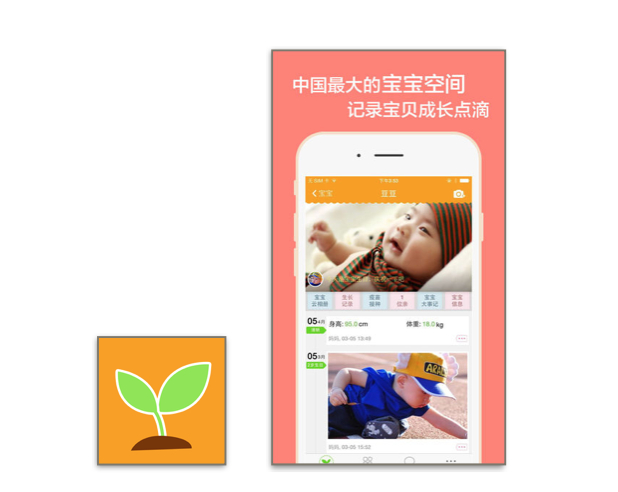
\includegraphics[width=0.80\textwidth]{qbb.png}
	\figcaption{亲宝宝}
	\label{fig:qinbaobao}
\end{figure}

亲宝宝是一个针对家长设计的app, 让亲友能够方便地记录宝宝的成长记录, 并且有一定的分享功能。

\begin{figure}[H]
	\centering
	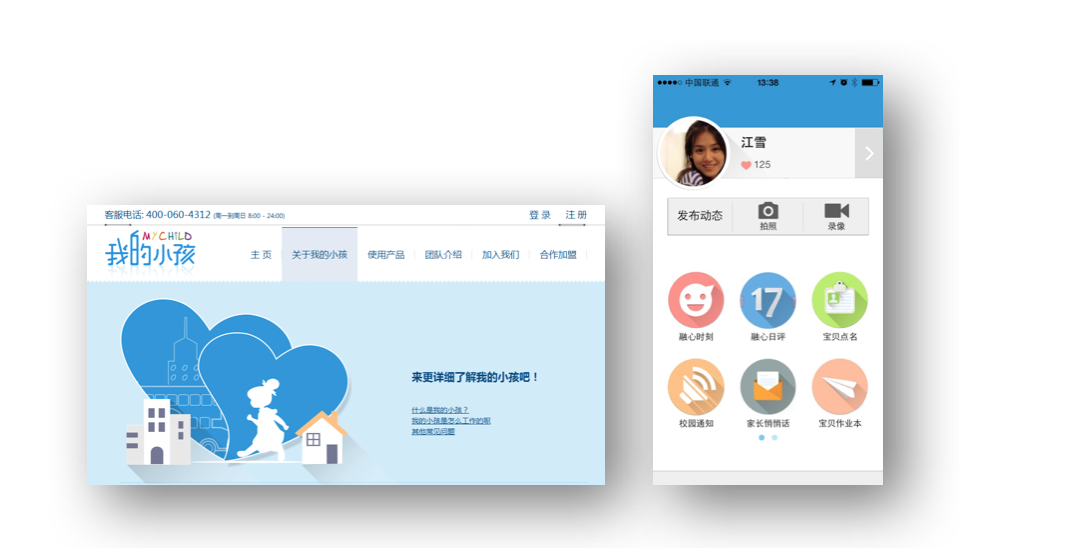
\includegraphics[width=0.80\textwidth]{hhz.png}
	\figcaption{好孩子}
	\label{fig:haohaizi}
\end{figure}

好孩子是一个面向幼儿园的人员管理系统, 有一定的社交功能, 但社交功能不强, 而且因为产品设计问题, 现在已经从itunes中下架, 而且只支持iphone端。



现在大部分幼儿园并没有对于人员的管理的信息系统, 老师和家长之间的交流方式主要通过微信,短信, QQ群。  


\section{课题主要内容与工作}

需要实现一个Web端, Web端的功能主要是管理, 面向用户为幼儿园管理层和幼儿园教师, 管理层主要功能:
	
	\begin{itemize}
		\item 	班级管理
		\begin{itemize}
			\item 班级中文件, 相册
			\item 班级中人员的转班, 入学
			\item 教师给父母发送学生的教师评语
			\item 班级中人员的转班, 入学
			\item 发布班级通知
		\end{itemize}
		
			\item 学校管理
		\begin{itemize}
			\item 学校中文件, 相册
			\item 学校中班级的管理
			\item 发布学校通知
		\end{itemize}
		 
		\item 不同教师拥有不同的权限
	
	\end{itemize}


在管理端的基础上, 实现App端, App端的功能主要是社交,老师, 管理者, 家长都会参与其中, 社交的主要功能有:

\begin{itemize}
	\item 每个用户都可以发布时间线
	\item 每个用户在自己主页看到同班用户发的时间线
	\item 可以在每个学校主页看到这个学校所有人发的时间线
	\item 可以提出加入班级申请
\end{itemize}


\section{论文结构}

在第一章, 我大致讲解了该产品的应用背景, 简述了应当具有的功能,在第二章, 我会介绍该产品使用到的技术和原则, 第三章, 我会进行详尽的需求分析。第四章, 会给出系统的概要设计。 在第五章, 详细介绍系统的设计与实现细节。第六章会大致讲解系统的测试, 最后第七章给出该项目的总结和展望。

